%!TEX root = ../Report.tex
%************************************************

% Detail design

\chapter{Introduction}
In this part the design of the end user application will be discussed in detail. Topics covered include the final selection of algorithms in the application, the design of the user interface, a high level overview of the data structures used, the functionality and features of the application and finally some additional considerations will be reviewed.

\chapter{Technology, Platform and Programming Language}
\section{Introduction}
Some algorithms and features lend themselves to being implemented more easily in certain languages than other. A programming language needs to be chosen that does not restrain the functionality of the application. 
The four languages with most support include:
\begin{enumerate}
\item Python
\item C\# (and other .NET languages)
\item Java
\item C++
\end{enumerate}

Machine learning libraries exist for all of the above mentioned languages. Python has poor support for rich user interfaces. Java is a good contender and is cross platform. Haskell has strong expressiveness and powerful language features.

\section{Trade-off study}

Thus in order to make a final selection a trade off study was conducted. Additional factors included in the trade-off study were the expressiveness and amount of features in a language and the cross platform compatibility. These features have a lower weighing.
Consideration is made to the end user and the user interface support is given the highest weighing.  

Thus the factors considered are:
\begin{itemize}
\item Development speed - Estimated amount of programmer time required in each language.
\item Available support and help - How easy it is to obtain help and support
\item Available machine learning and pattern recognition libraries. Implementation of some algorithms prove difficult.
\item \ac{UI} design and libraries - Availability of libraries to design a good user interface and experience
\item Cross platform compatibility - How well does the language, features and libraries run on other platforms
\item Expressiveness and features - Language features which ease development. Expressive languages facilitate advanced data structures and algorithms in few \ac{LOC}
\end{itemize}

% Table generated by Excel2LaTeX from sheet 'Sheet1'
\begin{table}[htbp]
  \centering
  \caption{Programming languages trade-off study}
    \begin{tabular}{rr|rrrrr}
    \toprule
          & Weight & C\#   & Java  & Python & C++   & Haskell \\
    \midrule
    Development speed & 0.5   & 8     & 7     & 8     & 5     & 9 \\
    Available support and help & 0.2   & 8     & 8     & 8     & 6     & 4 \\
    Machine learning libraries & 0.4   & 6     & 8     & 9     & 8     & 4 \\
    \acs{UI} design and libraries & 0.6   & 10    & 8     & 5     & 7     & 3 \\
    Cross platform compatibility & 0.2   & 6     & 10    & 10    & 10    & 10 \\
    Expressiveness and features & 0.4   & 7     & 6     & 8     & 5     & 10 \\
    \midrule
    Total & 2.3   & 18    & 17.5  & 17.4  & 15.1  & 14.7 \\
    \bottomrule
    \end{tabular}%
  \label{tab:languagetradeoff}%
\end{table}%

\section{Discussion}
Winner: \emph{C\#}\footnote{The algorithmic code is cross platform and can be run through Mono, even though the graphical front end developed in \ac{WPF} cannot.}

.NET languages facilitate the use of \ac{WPF} - a graphical system for rendering user interfaces, which will allow a rich user experience to be developed. Java and Python are good contenders.

C\# additionally has the following advantages:
\begin{enumerate}
\item Ability to easily create rich user interfaces.
\item C\# runs on the CLR and allows access to the large .NET library\footnote{Additionally the IKVM project allows access to Java libraries}
\item Powerful language constructs such as operator overloading, event handling, delegates, powerful multi-threading support and generics.
\end{enumerate}


\chapter{Selection of algorithms}
\section{Introduction}
In this chapter the selected algorithms for the end user application are chosen.
The algorithms for consideration are:
\begin{enumerate}
\item Melody generation with Genetic Algorithms.
\item Melody generation with Hidden Markov Models.
\item Accompaniment generation with Hidden Markov Models.
\item Accompaniment generation with a \ac{LSTM} network.
\item Accompaniment generation with a feed forward \ac{ANN}.
\item Instrumental generation with Markov Chains.
\end{enumerate}

The selection of algorithms will be done by means of elimination. Algorithms that yielded sub minimum results will not be selected for inclusion into the end user application.

\section{Trade-off studies}
For the final end-user application only a subset of algorithms will be chosen. In order to quantitatively select good algorithms a trade-off study will be done on the investigated algorithms. The factors considered are:
\begin{itemize}
\item Training time - The amount of time taken to train the algorithm on initial data.
\item Generation time - The amount of time the algorithm takes to produce a melody after it is trained.
\item Flexibility - How well the algorithm can accommodate different input data. How easily it can be extended or modified.
\item Pleasantness - Subjective measure of good a melody is.
\end{itemize}
% Table generated by Excel2LaTeX from sheet 'Sheet2'
\begin{table}[htbp]
  \centering
  \caption{Trade-off study for algorithms for melody generation}
    \begin{tabular}{rr|rrrr}
    \toprule
    \multicolumn{6}{c}{Melody generation} \\
    \midrule
          & Weight & GA    & FFANN & MC    & HMM \\
    \midrule 
    Training time & 0.3   & 10    & 4     & 8     & 5 \\
    Generation time & 0.6   & 4     & 7     & 8     & 7 \\
    Flexibility & 0.6   & 10    & 7     & 6     & 6 \\
    Pleasantness & 0.7   & 5     & 4     & 7     & 5 \\
          &       &       &       &       &  \\
          \bottomrule
    Total & 2.2   & 14.9  & 12.4  & 15.7  & 12.8 \\
    \bottomrule
    \end{tabular}%
  \label{tab:tomelgen}%
\end{table}%

Table \ref{tab:tomelgen} shows the trade-off study for algorithms for melody generation. Melody generation is simply the generation of a single track consisting of a list of notes. From the trade-off study we can see that the \ac{HMM} and \ac{FFANN} performed poorly and thus will not be selected.

% Table generated by Excel2LaTeX from sheet 'Sheet2'
\begin{table}[htbp]
  \centering
  \caption{Trade off study for algorithms for accompaniment generation}
    \begin{tabular}{rr|rrrr}
    \toprule
    \multicolumn{6}{c}{Accompaniment generation} \\
    \midrule
          & Weight & HMM   & FFANN & MM    & LSTM \\
    \midrule  
    Training time & 0.3   & 6     & 4     & 8     & 3 \\
    Generation time & 0.6   & 7     & 7     & 8     & 6 \\
    Flexibility & 0.6   & 6     & 7     & 6     & 5 \\
    Pleasantness & 0.7   & 3     & 5     & 6     & 3 \\
          &       &       &       &       &  \\
          \bottomrule
    Total & 2.2   & 11.7  & 13.1  & 15    & 9.6 \\
    \bottomrule
    \end{tabular}%
  \label{tab:toaccompgen}%
\end{table}%

Table \ref{tab:toaccompgen} indicates the trade-off study for algorithms for accompaniment generation. Accompaniment generation is a list of notes that have to accompany the main melody. From the trade-off study we can see that the \ac{HMM} and \ac{LSTM} performed poorly and thus will be excluded from the main application.

% Table generated by Excel2LaTeX from sheet 'Sheet3'
\begin{table}[htbp]
  \centering
  \caption{Comparison of frequency metric time and pleasantness}
    \begin{tabular}{r|rr}
    \toprule
          & Time (ms) & Pleasantness \\
    \midrule
    Chromatic Tone & 8992  & 4 \\
    Chromatic Tone Distance & 11017 & 5 \\
    Chromatic Tone Duration & 13688 & 5 \\
    Melodic Bigram & 3900  & 5 \\
    Melodic Interval & 9037  & 5 \\
    Pitch & 14001 & 4 \\
    Pitch Distance & -     & - \\
    Rhythm & 367   & 4 \\
    Rhythmic Bigram & 4729  & 7 \\
    Rhythmic Interval & 5501  & 6 \\
    \bottomrule
    \end{tabular}%
  \label{tab:fmetrictimepleasant}%
\end{table}%


For the frequency metrics to be used with the cosine similarity fitness function we refer to table \ref{tab:metriccomp}. The pleasantness and time for each metric is repeated in table \ref{tab:fmetrictimepleasant} for convenience. The Pitch Distance metric was excluded as it took too long. The chromatic tone, pitch and rhythm metrics will also be excluded as all scored low pleasantness. 


\section{Conclusion}
From the trade-off study the selected algorithms were chosen.
In summary, the selected algorithms for the end-user application were:
\begin{enumerate}
\item Genetic Algorithms for melody generation.
\item Markov Chains for melody generation (with percussion support).
\item Feed Forward Artificial Neural Network for accompaniment generation.
\item Markov Model for accompaniment generation.
\end{enumerate}

Only the cosine similarity fitness function will be used, as the \ac{NCD} fitness function performed poorly. The metrics for the cosine similarity fitness function were selected as:
\begin{enumerate}
\item Chromatic Tone Distance
\item Chromatic Tone Duration
\item Melodic Bigram
\item Melodic Interval
\item Rhythmic Bigram
\item Rhythmic Interval
\end{enumerate}

Using trade-off studies the worst results were eliminated from all algorithms.

\chapter{Features and Functionality}
The main goal of the application is to generate melodies according to a certain styles. The user is to select a certain category of music and the application will generate a musical piece in that style. The premise is to generate the melodies in a certain style using machine learning techniques that will use the data present in the corpus of MIDI files. 

Since training machine learning algorithms take up a lot of time it is not feasible to train the algorithm on the fly. Training will take place beforehand and the resulting data structure of the algorithm will be cached to a file. 
For example a Neural Network will save its topology and weights to a file; this allows the application to load the file, present inputs to the neural network and output a result without spending time learning the optimal weights for the network.

Additional features would be to allow the user to save a generated melody to a file (in \ac{MIDI} or a custom file format), load and play an existing \ac{MIDI} file (for comparison or other aims), re-randomize a generated composition and view more information or properties of the generated music piece.

The application is to be used by end users which do not have background on machine learning. The application is to be as user-friendly as possible while still having flexibility in composing songs. The user interface is to visually display the song and playback of it. Playback functionality such as playing and stopping a song are mandatory.

To summarize, the application will:
\begin{enumerate}
\item Implement the selected algorithms and allow them to be used for song generation.
\item Allow saving and loading of \ac{MIDI} files
\item Generate a monophonic melody according to a certain style. Allow the user to select which algorithm to use and adjust high level parameters
\item Playback functionality including playing, pausing and stop a song. 
\item Feature a user friendly interface.
\item Visually display the generated melody.
\item Allow the user to randomize the song based on the selected settings.
\item Cache machine learning data to improve performance of the application.
\end{enumerate}

\chapter{Graphical user interface}

\section{Introduction}

In this chapter the design of the graphical user interface is presented, along with the features and functionality of the application.

As mentioned above the user interface is to have the following features
\begin{itemize}
\item Visually display the generated song.
\item Selecting the category of melodies to be generated.
\item Select algorithm and high level parameters.
\item Buttons to allow for saving, loading, pausing, pausing, stopping and playing of songs.
\end{itemize}

The user interface will be developed using \ac{WPF} and \ac{XAML}.

\section{Playback}

\begin{figure}
\centerline{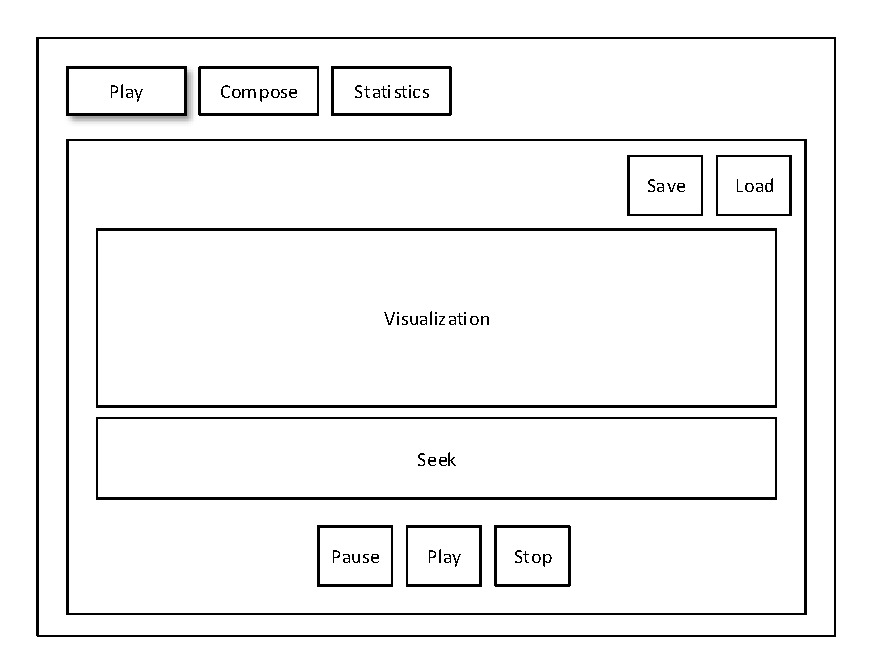
\includegraphics[width=400px]{../images/ui_play.pdf}}
\caption{User interface for playback functionality}
\label{ims:uiplay}
\end{figure}



Figure \ref{ims:uiplay} indicates the starting interface of the application. This interface provides controls for playback functionality, is responsible for displaying a visual of the song being currently played, provides saving and loading functionality and allows the user to randomize the current song using the parameters set in the compose view.

\section{Composition}
\begin{figure}
\centerline{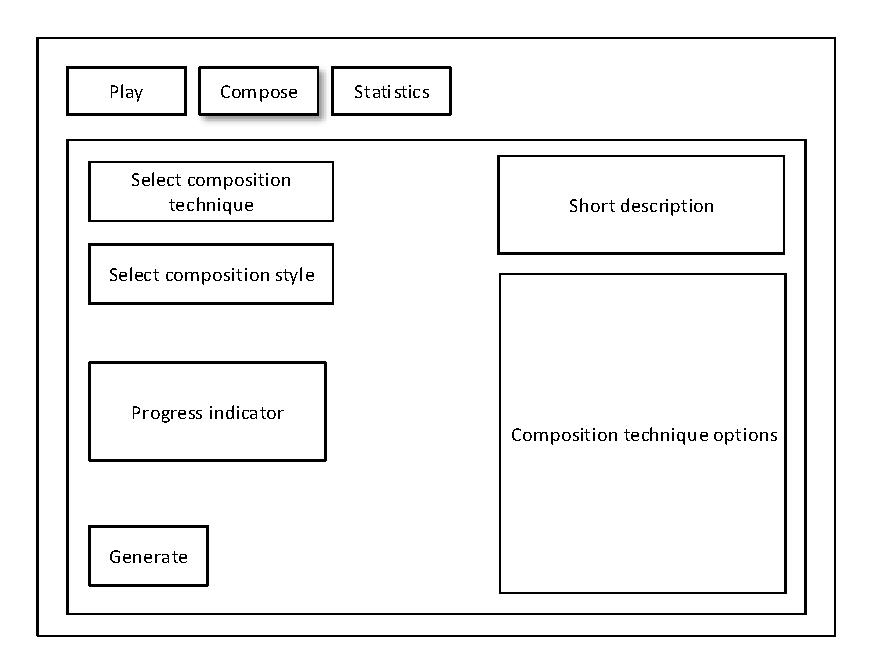
\includegraphics[width=400px]{../images/ui_compose.pdf}}
\caption{User interface for composition functionality}
\label{ims:uicompose}
\end{figure}


The interface as shown in figure \ref{ims:uicompose} allows the user to select the music style or category for music to be generated in. A track is a sequence of notes played in a particular instrument. A user is able to add new tracks using the provided button, which takes them to a new window as in figure \ref{ims:uitrack}. If a user double clicks on a specific track the frequency metrics of the track are shown as in figure \ref{ims:uimetrics}.


\section{Track generation}

Figure \ref{ims:uitrack} allows the user to generate a track using a specific technique. This interface allows the user to select the type of technique for track generation and also displays the progress. Once a track is generated it can be added to the list of tracks as in figure \ref{ims:uicompose}.

\begin{figure}
\centerline{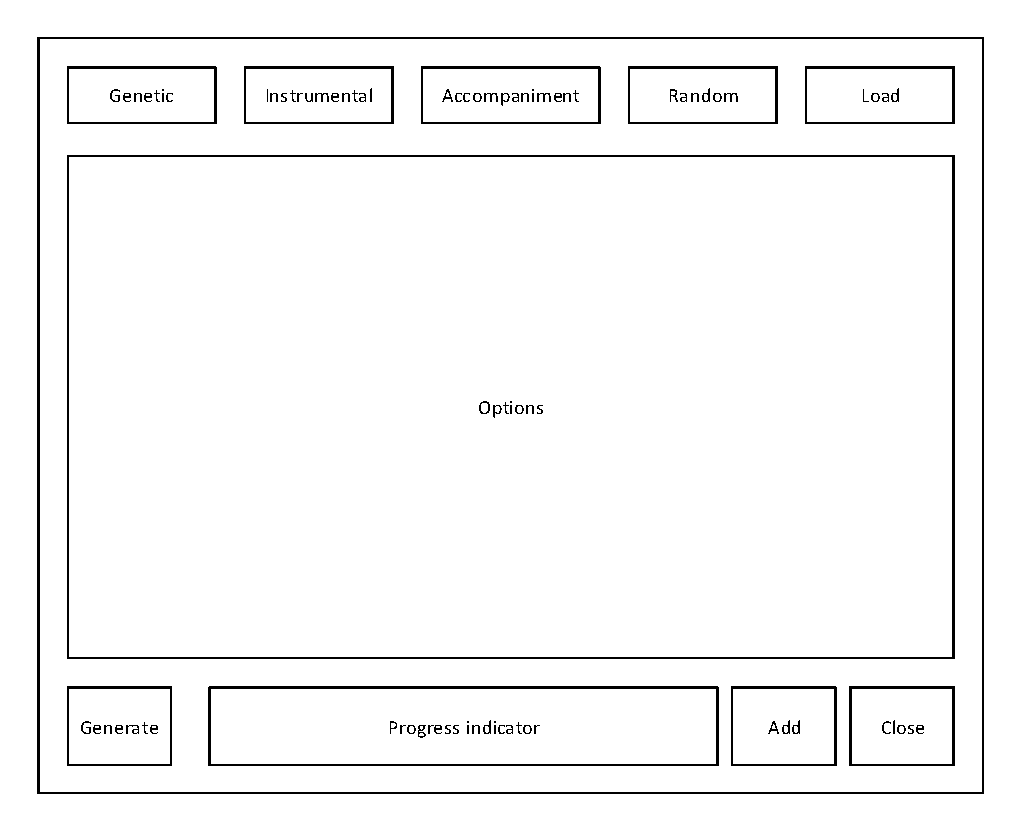
\includegraphics[width=400px]{../images/ui_track.pdf}}
\caption{User interface for melody generation}
\label{ims:uitrack}
\end{figure}



\section{Statistics}

Figure \ref{ims:uimetrics} displays a list of frequency metrics about the track selected. An example metric is the frequency of musical intervals within a melody ($\text{mi} = |p_i - p_{i-1}|$, where $p_i$ is the pitch at index $i$); more information about frequency metrics can be found in section \label{chap:metrics}.

\begin{figure}
\centerline{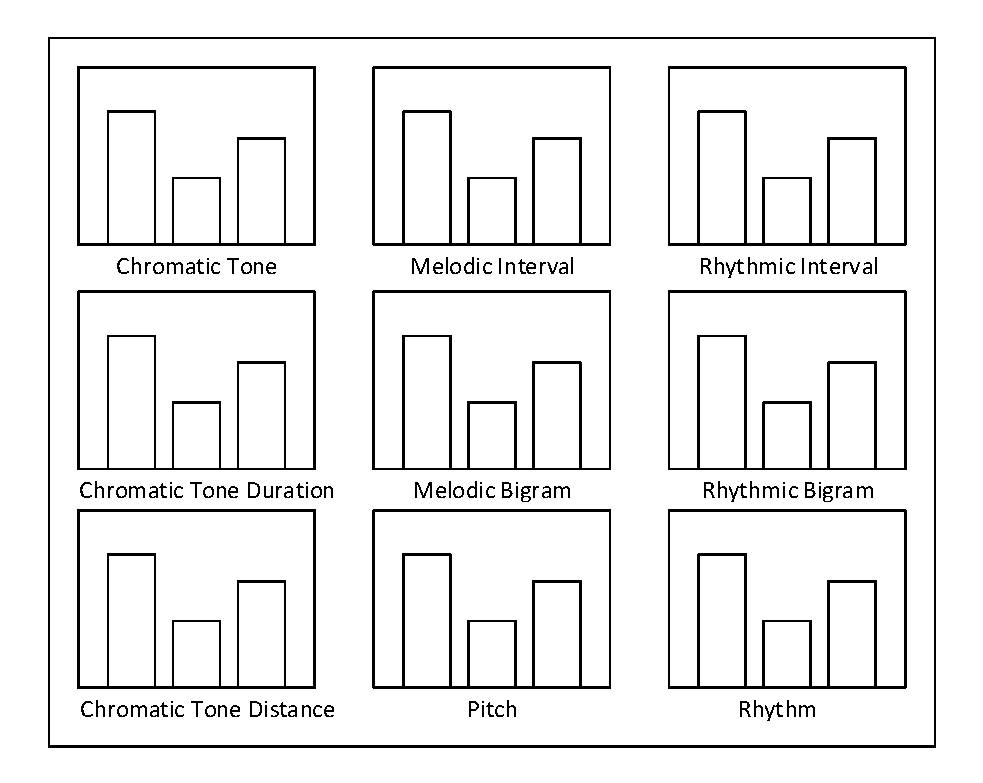
\includegraphics[width=400px]{../images/ui_metrics.pdf}}
\caption{User interface for displaying metrics of a melody}
\label{ims:uimetrics}
\end{figure}

 
\section{Visualization}
The visualization blocks in figures \ref{ims:uicompose} and \ref{ims:uitrack} will be a simple visual displaying the notes over time. 

%A simplified music sheet representation will be used, something in the vein of figure \ref{ims:uiharrymusicsheet}.

\begin{figure}
\centerline{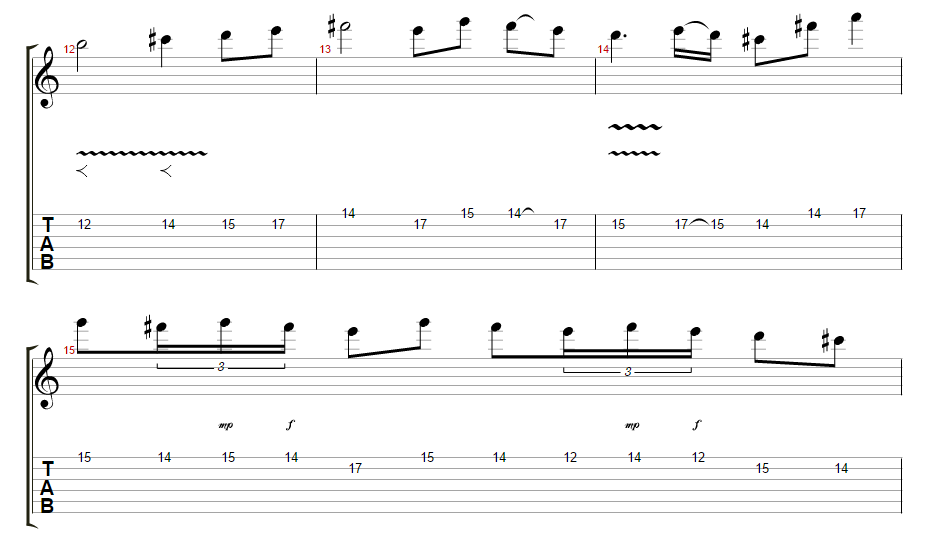
\includegraphics[width=400px]{../images/alphatab_example.png}}
\caption{Example of a music sheet rendered with alphatab}
\label{ims:alphatab}
\end{figure}

AlphaTab is a cross platform music notation and guitar tablature rendering library. It is the only music notation library available on C\# which will fit the need for visualization of notes required.
Figure \ref{ims:alphatab} indicates a music sheet rendered with Alphatab. Note that Alphatab is geared towards guitarists and provides a lot more information which is unwanted for a simple visualization. 

Since the library is open source it will be modified to suit our needs. Guitar tabs, timing information, lyrics and any other excessive information will be removed. In addition it is necessary to show which note is currently played when a melody is played. The active note will be displayed in red.

\begin{figure}
\centerline{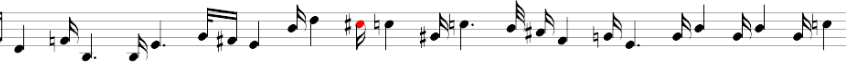
\includegraphics[width=300px]{../images/music_sheet_visualization.png}}
\caption{Desired notes visualization}
\label{ims:uiharrynotesvisualization}
\end{figure}

Figure \ref{ims:uiharrynotesvisualization} displays the designed simple notes visualization required for the application. Alphatab will be modified in order to produce a result similar to this.


%\begin{figure}
%\centerline{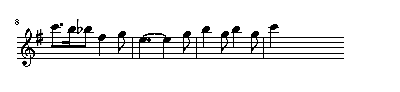
\includegraphics[width=400px]{../images/ui_visualization.pdf}}
%\caption{Visualization of notes}
%\label{ims:uiharrymusicsheet}
%\end{figure}



\section{State control}

\begin{figure}
\centerline{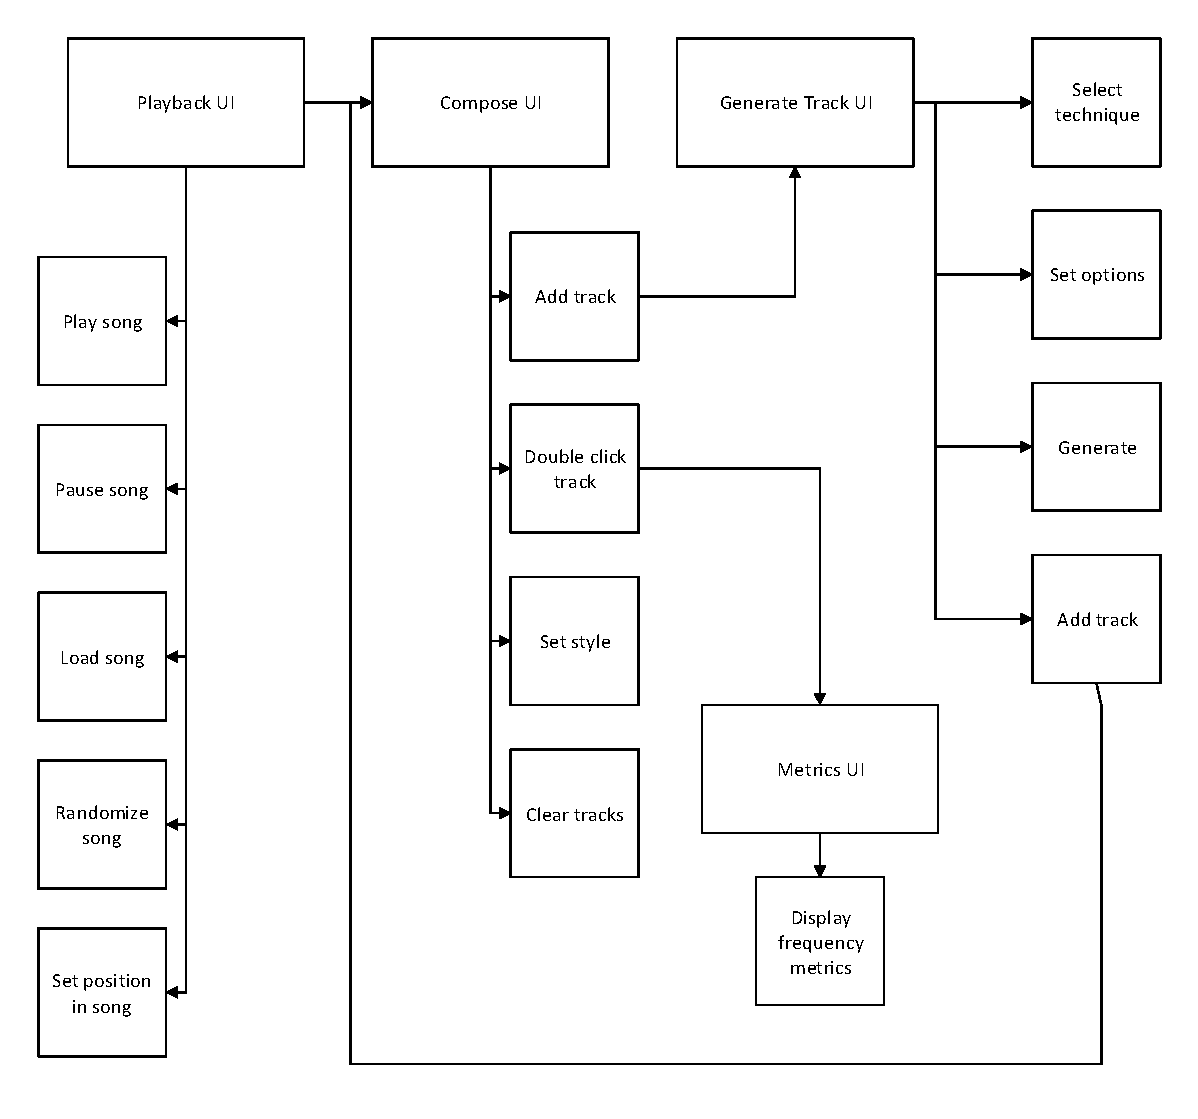
\includegraphics[width=400px]{../images/ui_control_blockdiagram.pdf}}
\caption{State diagram of the user interface}
\label{ims:uiflow}
\end{figure}

Figure \ref{ims:uiflow} shows the state diagram of the user interface. 
From the figure it can be seen that the Playback UI controls playback of a single composition. From the composition UI the necessary tools and functionality can be accessed to create new melodies.


% Functionality and features
% Design
\chapter{Final considerations}